% Options for packages loaded elsewhere
\PassOptionsToPackage{unicode}{hyperref}
\PassOptionsToPackage{hyphens}{url}
\documentclass[
  twocolumn]{article}
\usepackage{xcolor}
\usepackage[margin=0.95in]{geometry}
\usepackage{amsmath,amssymb}
\setcounter{secnumdepth}{-\maxdimen} % remove section numbering
\usepackage{iftex}
\ifPDFTeX
  \usepackage[T1]{fontenc}
  \usepackage[utf8]{inputenc}
  \usepackage{textcomp} % provide euro and other symbols
\else % if luatex or xetex
  \usepackage{unicode-math} % this also loads fontspec
  \defaultfontfeatures{Scale=MatchLowercase}
  \defaultfontfeatures[\rmfamily]{Ligatures=TeX,Scale=1}
\fi
\usepackage{lmodern}
\ifPDFTeX\else
  % xetex/luatex font selection
\fi
% Use upquote if available, for straight quotes in verbatim environments
\IfFileExists{upquote.sty}{\usepackage{upquote}}{}
\IfFileExists{microtype.sty}{% use microtype if available
  \usepackage[]{microtype}
  \UseMicrotypeSet[protrusion]{basicmath} % disable protrusion for tt fonts
}{}
\makeatletter
\@ifundefined{KOMAClassName}{% if non-KOMA class
  \IfFileExists{parskip.sty}{%
    \usepackage{parskip}
  }{% else
    \setlength{\parindent}{0pt}
    \setlength{\parskip}{6pt plus 2pt minus 1pt}}
}{% if KOMA class
  \KOMAoptions{parskip=half}}
\makeatother
\usepackage{color}
\usepackage{fancyvrb}
\newcommand{\VerbBar}{|}
\newcommand{\VERB}{\Verb[commandchars=\\\{\}]}
\DefineVerbatimEnvironment{Highlighting}{Verbatim}{commandchars=\\\{\}}
% Add ',fontsize=\small' for more characters per line
\usepackage{framed}
\definecolor{shadecolor}{RGB}{248,248,248}
\newenvironment{Shaded}{\begin{snugshade}}{\end{snugshade}}
\newcommand{\AlertTok}[1]{\textcolor[rgb]{0.94,0.16,0.16}{#1}}
\newcommand{\AnnotationTok}[1]{\textcolor[rgb]{0.56,0.35,0.01}{\textbf{\textit{#1}}}}
\newcommand{\AttributeTok}[1]{\textcolor[rgb]{0.13,0.29,0.53}{#1}}
\newcommand{\BaseNTok}[1]{\textcolor[rgb]{0.00,0.00,0.81}{#1}}
\newcommand{\BuiltInTok}[1]{#1}
\newcommand{\CharTok}[1]{\textcolor[rgb]{0.31,0.60,0.02}{#1}}
\newcommand{\CommentTok}[1]{\textcolor[rgb]{0.56,0.35,0.01}{\textit{#1}}}
\newcommand{\CommentVarTok}[1]{\textcolor[rgb]{0.56,0.35,0.01}{\textbf{\textit{#1}}}}
\newcommand{\ConstantTok}[1]{\textcolor[rgb]{0.56,0.35,0.01}{#1}}
\newcommand{\ControlFlowTok}[1]{\textcolor[rgb]{0.13,0.29,0.53}{\textbf{#1}}}
\newcommand{\DataTypeTok}[1]{\textcolor[rgb]{0.13,0.29,0.53}{#1}}
\newcommand{\DecValTok}[1]{\textcolor[rgb]{0.00,0.00,0.81}{#1}}
\newcommand{\DocumentationTok}[1]{\textcolor[rgb]{0.56,0.35,0.01}{\textbf{\textit{#1}}}}
\newcommand{\ErrorTok}[1]{\textcolor[rgb]{0.64,0.00,0.00}{\textbf{#1}}}
\newcommand{\ExtensionTok}[1]{#1}
\newcommand{\FloatTok}[1]{\textcolor[rgb]{0.00,0.00,0.81}{#1}}
\newcommand{\FunctionTok}[1]{\textcolor[rgb]{0.13,0.29,0.53}{\textbf{#1}}}
\newcommand{\ImportTok}[1]{#1}
\newcommand{\InformationTok}[1]{\textcolor[rgb]{0.56,0.35,0.01}{\textbf{\textit{#1}}}}
\newcommand{\KeywordTok}[1]{\textcolor[rgb]{0.13,0.29,0.53}{\textbf{#1}}}
\newcommand{\NormalTok}[1]{#1}
\newcommand{\OperatorTok}[1]{\textcolor[rgb]{0.81,0.36,0.00}{\textbf{#1}}}
\newcommand{\OtherTok}[1]{\textcolor[rgb]{0.56,0.35,0.01}{#1}}
\newcommand{\PreprocessorTok}[1]{\textcolor[rgb]{0.56,0.35,0.01}{\textit{#1}}}
\newcommand{\RegionMarkerTok}[1]{#1}
\newcommand{\SpecialCharTok}[1]{\textcolor[rgb]{0.81,0.36,0.00}{\textbf{#1}}}
\newcommand{\SpecialStringTok}[1]{\textcolor[rgb]{0.31,0.60,0.02}{#1}}
\newcommand{\StringTok}[1]{\textcolor[rgb]{0.31,0.60,0.02}{#1}}
\newcommand{\VariableTok}[1]{\textcolor[rgb]{0.00,0.00,0.00}{#1}}
\newcommand{\VerbatimStringTok}[1]{\textcolor[rgb]{0.31,0.60,0.02}{#1}}
\newcommand{\WarningTok}[1]{\textcolor[rgb]{0.56,0.35,0.01}{\textbf{\textit{#1}}}}
\usepackage{longtable,booktabs,array}
\usepackage{calc} % for calculating minipage widths
% Correct order of tables after \paragraph or \subparagraph
\usepackage{etoolbox}
\makeatletter
\patchcmd\longtable{\par}{\if@noskipsec\mbox{}\fi\par}{}{}
\makeatother
% Allow footnotes in longtable head/foot
\IfFileExists{footnotehyper.sty}{\usepackage{footnotehyper}}{\usepackage{footnote}}
\makesavenoteenv{longtable}
\usepackage{graphicx}
\makeatletter
\newsavebox\pandoc@box
\newcommand*\pandocbounded[1]{% scales image to fit in text height/width
  \sbox\pandoc@box{#1}%
  \Gscale@div\@tempa{\textheight}{\dimexpr\ht\pandoc@box+\dp\pandoc@box\relax}%
  \Gscale@div\@tempb{\linewidth}{\wd\pandoc@box}%
  \ifdim\@tempb\p@<\@tempa\p@\let\@tempa\@tempb\fi% select the smaller of both
  \ifdim\@tempa\p@<\p@\scalebox{\@tempa}{\usebox\pandoc@box}%
  \else\usebox{\pandoc@box}%
  \fi%
}
% Set default figure placement to htbp
\def\fps@figure{htbp}
\makeatother
\setlength{\emergencystretch}{3em} % prevent overfull lines
\providecommand{\tightlist}{%
  \setlength{\itemsep}{0pt}\setlength{\parskip}{0pt}}
\usepackage{tabularx}
\usepackage{booktabs}
\usepackage{longtable}
\usepackage{array}
\usepackage{multirow}
\usepackage{wrapfig}
\usepackage{float}
\usepackage{colortbl}
\usepackage{pdflscape}
\usepackage{tabu}
\usepackage{threeparttable}
\usepackage{threeparttablex}
\usepackage[normalem]{ulem}
\usepackage{makecell}
\usepackage{xcolor}
\usepackage{bookmark}
\IfFileExists{xurl.sty}{\usepackage{xurl}}{} % add URL line breaks if available
\urlstyle{same}
\hypersetup{
  hidelinks,
  pdfcreator={LaTeX via pandoc}}

\author{}
\date{\vspace{-2.5em}}

\begin{document}

\section{\texorpdfstring{\textit{How does violating homoscedasticity affect inference in linear regression?}}{}}\label{section}

Yanqi Huang, MS Student\footnote{Department of Biostatistics and Informatics, Colorado School of Public Health, University of Colorado Anschutz Medical Campus, Aurora, CO}

\subsection{Abstract}\label{abstract}

Ordinary least squares (OLS) regression relies on the assumption of constant error variance. This simulation study shows that while OLS estimates remain unbiased under heteroscedasticity, model-based standard errors underestimate true variability, leading to confidence intervals with poor coverage. These results highlight the need to account for heteroscedasticity to ensure valid inference.

\subsection{Introduction}\label{introduction}

Ordinary least squares (OLS) regression is widely used to explore relationships between explanatory factors and an outcome variable. For example, in biomedical research, it is often applied to assess associations between risk factors and health outcomes. The key assumptions of OLS include linearity, normality of errors, and homoscedasticity.The purpose of this study is to evaluate how varying levels of heteroscedasticity affect inference in OLS regression using simulation.

\subsection{Motivating Problem}\label{motivating-problem}

In practice, the assumption of homoscedasticity is frequently overlooked when fitting linear regression models. However, violations of this assumption can have a greater impact on the validity of regression results than violations of normality \(^1\). This simulation study examined the impact of mild, moderate, and strong levels of heteroscedasticity on bias, model-based standard error(SE), empirical standard error, their relative error and confidence interval (CI) coverage in ordinary OLS regression.

\subsection{Simulation Set-Up}\label{simulation-set-up}

To evaluate how key performance metrics vary under increasing heteroscedasticity, the simulation was designed as follows:

\begin{enumerate}
\def\labelenumi{\arabic{enumi}.}
\item
  The predictor \(x_i\) is generated from a uniform distribution \(x_i \sim \text{Uniform}(1, 6)\) with a sample size of \(n = 100\) {[}3{]}.
\item
  \(\mu_x\) denote the mean of \(x\). The error variance is defined as a function of \(x\), with parameter \(c\) controlling the degree of heteroscedasticity:

  \[
  \varepsilon_i \sim \mathcal{N}\!\left(0,\;
  \frac{\exp\{c(x_i - \mu_x)\}}
  {\mathbb{E}\!\left[\exp\{c(x_i - \mu_x)\}\right]}\right)
  \]

  \begin{itemize}
  \item
    \(c=0\) (homoscedastic baseline): The variance simplifies to \(1\) for all \(x_i\), giving\[
    \varepsilon_i \sim \mathcal{N}(0,1)
    \]
  \item
    \(c=0.3\) (mild heteroscedasticity): The variance increases modestly with \$\(x_i\), producing mild departures from constant variance.
  \item
    \(c=1\) (Moderate heteroscedasticity): Variance grows more noticeably across the range of \(x_i\), yielding moderate heteroscedasticity.
  \item
    \(c=6\) (Strong heteroscedasticity): Variance differs substantially with \(x_i\), representing strong heteroscedasticity.

    Residual plots against fitted values for each scenario are shown in Figure 1 to illustrate the increasing degree of heteroscedasticity.
  \end{itemize}
\item
  The response variable is defined as\\
  \[
  y_i = 14 + 0.4x_i + \varepsilon_i
  \] with the true slope \(\beta_1 = 0.4\) {[}3{]}.
\item
  Each scenario is replicated 1000 times, consistent with the average number of iterations used in previous studies {[}3{]}.
\end{enumerate}

Residual plots in Figure \ref{fig:1} show that increasing \(c\) produces greater spread of residuals with \(\hat{y}\), reflecting progressively stronger heteroscedasticity.

\begin{figure}
\centering
\pandocbounded{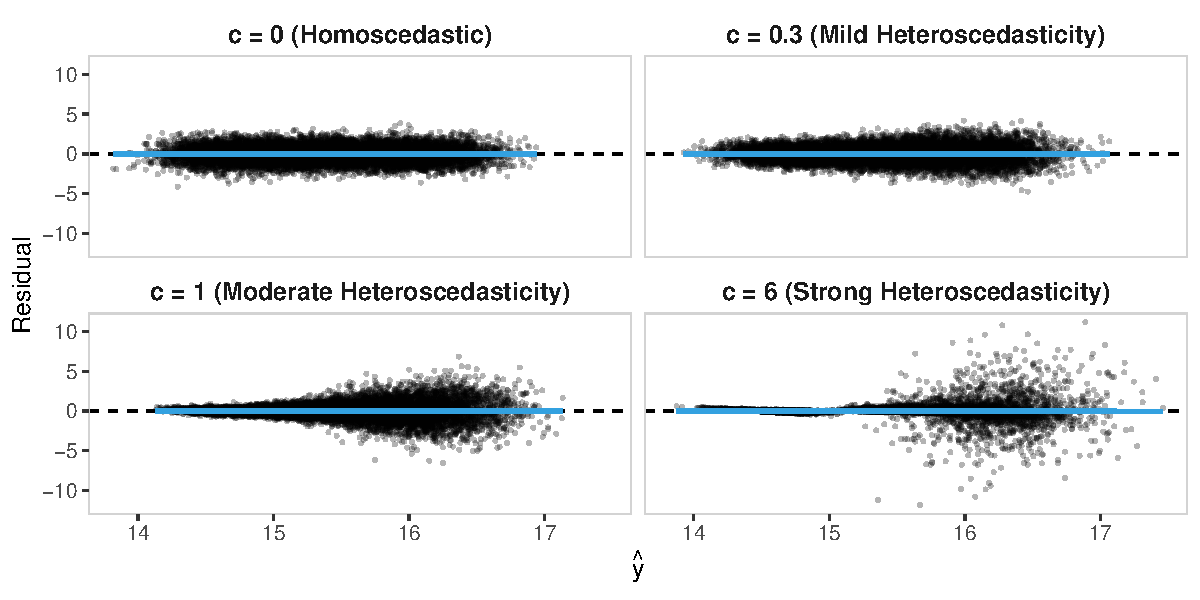
\includegraphics[keepaspectratio]{yanqi_simulation_midterm_shell_files/figure-latex/unnamed-chunk-1-1.pdf}}
\caption{\label{fig:unnamed-chunk-1}Residuals vs.~fitted values for OLS regression under Homoscedasticity(c=0) and increasing levels of heteroscedasticity(c=0.3,1,6)}
\end{figure}

To introduce heteroscedasticity, the error variance is modeled as a function of \(x\), with larger values of \(c\) producing more uneven variability across \(x\). Without adjustment, both the average error variance \(\mathbb{E}[\operatorname{Var}(\varepsilon_i)]\) and the variance of the outcome \(y\) increase as \(c\) grows, confounding the effect of heteroscedasticity with overall noise. To address this, the variance function is normalized by \(\mathbb{E}[\exp\{c(x_i - \mu_x)\}]\), which fixes the average error variance at \(1\). This normalization isolates the impact of heteroscedasticity itself while keeping the total noise level constant, allowing fair comparison between homoscedastic and heteroscedastic settings.

\begin{table}[H]
\centering
\caption{\label{tab:unnamed-chunk-2}Variance of $Y$ and expected error variance $\mathbb{E}[\mathrm{Var}(\varepsilon\mid X)]$ across heteroscedasticity levels ($c$): normalized vs. unnormalized.}
\centering
\resizebox{\ifdim\width>\linewidth\linewidth\else\width\fi}{!}{
\fontsize{10}{12}\selectfont
\begin{tabular}[t]{lrrrr}
\toprule
\multicolumn{1}{c}{ } & \multicolumn{2}{c}{Normalized} & \multicolumn{2}{c}{Unnormalized} \\
\cmidrule(l{3pt}r{3pt}){2-3} \cmidrule(l{3pt}r{3pt}){4-5}
$c$ & $\mathrm{Var}(Y)$ & $\mathbb{E}[\mathrm{Var}(\varepsilon\mid X)]$ & $\mathrm{Var}(Y)$ & $\mathbb{E}[\mathrm{Var}(\varepsilon\mid X)]$\\
\midrule
0 & 1 & 1 & 1 & 1\\
0.3 & 1 & 1 & 1 & 1\\
1 & 1 & 1 & 3 & 2\\
6 & 1 & 1 & 110319 & 109623\\
\bottomrule
\end{tabular}}
\end{table}

The results will be presented graphically across the grid of \(c\) values and summarized in a table showing the bias, model-based SE, empirical SE, relative error in model SE and CI coverage of \(\hat{\beta}_1\).

\subsection{Results}\label{results}

Figure 1 summarizes the effect of increasing heteroscedasticity(parameter c) on the estimation of \(\hat{\beta}_1\), with 95\% Monte Carlo confidence intervals. Across all values of c, the bias remained close to zero, confirming that OLS produced unbiased slope estimates. In contrast, the variability metrics showed divergent patterns: the empirical standard error increased steadily from 0.069 under homoscedasticity (c=0) to 0.111 at c=6, while the model-based standard error decreased slightly from 0.070 to 0.066. This discrepancy led to progressively larger underestimation of variability, with the relative error in the model-based standard error reaching -40.9\% at c=6. Consequently, confidence interval coverage declined from near the nominal 95\% (94.4\%) under homoscedasticity to only 76.5\% under strong heteroscedasticity.

\begin{figure}
\centering
\pandocbounded{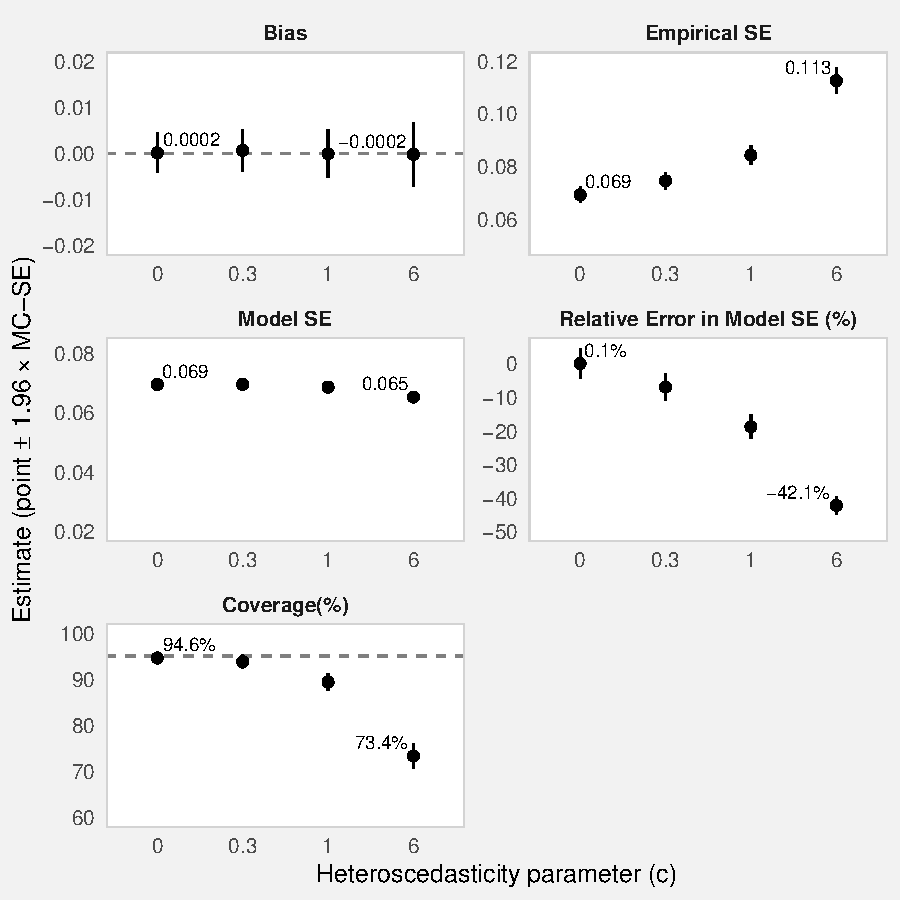
\includegraphics[keepaspectratio]{yanqi_simulation_midterm_shell_files/figure-latex/unnamed-chunk-3-1.pdf}}
\caption{\label{fig:unnamed-chunk-3}Metrics with 95\% Monte Carlo Confidence Intervals across Levels of Heteroscedasticity}
\end{figure}

Table 1 provides the detailed numerical results corresponding to Figure 1, including point estimates with Monte Carlo standard errors. The table highlights that bias was consistently negligible, with all estimates within ±0.004. However, empirical standard errors grew substantially larger than their model-based counterparts as heteroscedasticity increased. For example, at c=6 the empirical standard error was 0.111 (±0.002) compared to a model-based standard error of only 0.066 (±0.001). This mismatch explains the sharp decline in confidence interval coverage, which fell nearly 20 percentage points below the nominal level.

\begin{table}[H]
\centering
\caption{\label{tab:unnamed-chunk-4}Simulation results for OLS regression under heteroscedasticity with Monte Carlo standard errors (in parentheses)}
\centering
\fontsize{9}{11}\selectfont
\begin{tabular}[t]{cccccc}
\toprule
c & Bias & \makecell{Model\\SE} & \makecell{Empirical\\SE} & \makecell{Relative\\error in\\model SE\\(\%)} & \makecell{CI\\Coverage\\(\%)}\\
\midrule
0 & \makecell{0.0002 \\ (±0.002)} & \makecell{0.069 \\ (±0.000)} & \makecell{0.069 \\ (±0.002)} & \makecell{0.1 \\ (±2.3)} & \makecell{94.6 \\ (±0.7)}\\
0.3 & \makecell{0.0007 \\ (±0.002)} & \makecell{0.070 \\ (±0.000)} & \makecell{0.075 \\ (±0.002)} & \makecell{-6.9 \\ (±2.1)} & \makecell{93.8 \\ (±0.8)}\\
1 & \makecell{-0.0000 \\ (±0.003)} & \makecell{0.069 \\ (±0.000)} & \makecell{0.084 \\ (±0.002)} & \makecell{-18.7 \\ (±1.8)} & \makecell{89.4 \\ (±1.0)}\\
6 & \makecell{-0.0002 \\ (±0.004)} & \makecell{0.065 \\ (±0.001)} & \makecell{0.113 \\ (±0.003)} & \makecell{-42.1 \\ (±1.4)} & \makecell{73.4 \\ (±1.4)}\\
\bottomrule
\end{tabular}
\end{table}

\subsection{Conclusion}\label{conclusion}

These simulations show that while OLS slope estimates remain unbiased under heteroscedasticity, inference based on model-based standard errors is unreliable. As heteroscedasticity increased, empirical variability rose but model-based standard errors fell slightly, leading to confidence intervals with coverage up to 20 percentage points below nominal levels.

Thus, OLS-based inference under heteroscedasticity gives overly optimistic precision. Robust alternatives---such as heteroscedasticity-consistent standard errors or alternative models---should be used to ensure valid inference.

There are limitations to this study. Only one covariate distribution, a fixed sample size, and a single form of heteroscedasticity were examined. Future work could investigate other covariate distributions, larger sample sizes, and different error variance structures.

Careful consideration of error variance assumptions is critical in regression analysis, as violations can lead to misleadingly narrow confidence intervals and incorrect scientific conclusions.

\newpage
\onecolumn

\subsection{References}\label{references}

\vspace{2mm}

\phantomsection\label{refs}

\subsection{Code Appendix}\label{code-appendix}

\begin{Shaded}
\begin{Highlighting}[]
\NormalTok{knitr}\SpecialCharTok{::}\NormalTok{opts\_chunk}\SpecialCharTok{$}\FunctionTok{set}\NormalTok{(}\AttributeTok{echo =} \ConstantTok{TRUE}\NormalTok{)}
\CommentTok{\#bibliography: kaizer\_simulation\_sample1.bib}
\CommentTok{\#csl: alex\_vancouver.csl}
\DocumentationTok{\#\# ================================}
\DocumentationTok{\#\# 0. Load needed packages and data}
\DocumentationTok{\#\# ================================}
\CommentTok{\# Helper function: install if not already available}
\NormalTok{load\_or\_install }\OtherTok{\textless{}{-}} \ControlFlowTok{function}\NormalTok{(pkg)\{}
  \ControlFlowTok{if}\NormalTok{ (}\SpecialCharTok{!}\FunctionTok{requireNamespace}\NormalTok{(pkg, }\AttributeTok{quietly =} \ConstantTok{TRUE}\NormalTok{)) \{}
    \FunctionTok{install.packages}\NormalTok{(pkg)}
\NormalTok{  \}}
  \FunctionTok{library}\NormalTok{(pkg, }\AttributeTok{character.only =} \ConstantTok{TRUE}\NormalTok{)}
\NormalTok{\}}

\CommentTok{\# List of needed packages}
\NormalTok{packages }\OtherTok{\textless{}{-}} \FunctionTok{c}\NormalTok{(}\StringTok{"dplyr"}\NormalTok{, }\StringTok{"ggplot2"}\NormalTok{,  }\StringTok{"kableExtra"}\NormalTok{, }\StringTok{"webshot2"}\NormalTok{,}\StringTok{"magick"}\NormalTok{,}\StringTok{"knitr"}\NormalTok{,}\StringTok{"tidyverse"}\NormalTok{,}\StringTok{"tidyr"}\NormalTok{,}\StringTok{"ggh4x"}\NormalTok{)}
\CommentTok{\# Load or install each}
\FunctionTok{lapply}\NormalTok{(packages, load\_or\_install)}


\CommentTok{\# Load simulation results}
\NormalTok{path }\OtherTok{\textless{}{-}} \StringTok{"\textasciitilde{}/Library/CloudStorage/Dropbox/School/CU/fall 2025/BIOS 6618 adv biostatistical method/midterm simulation/simulation{-}study/"}
\NormalTok{fits\_file }\OtherTok{\textless{}{-}} \StringTok{\textquotesingle{}/data/2025{-}10{-}22\_optimized{-}seed{-}best{-}param{-}centered{-}log{-}linear{-}fits\_ols{-}heteroscedasticity{-}simulation\_n100\_reps1000\_seed1234\_c0{-}0.3{-}1{-}6.rds\textquotesingle{}}
\NormalTok{simulated\_data\_file }\OtherTok{\textless{}{-}} \StringTok{\textquotesingle{}/data/2025{-}10{-}22\_optimized{-}seed{-}best{-}param{-}centered{-}log{-}linear{-}datasets\_ols{-}heteroscedasticity{-}simulation\_n100\_reps1000\_seed1234\_c0{-}0.3{-}1{-}6.rds\textquotesingle{}}
\NormalTok{fits }\OtherTok{\textless{}{-}} \FunctionTok{readRDS}\NormalTok{(}\FunctionTok{paste0}\NormalTok{(path, fits\_file))}
\NormalTok{simulated\_data }\OtherTok{\textless{}{-}} \FunctionTok{readRDS}\NormalTok{(}\FunctionTok{paste0}\NormalTok{(path, simulated\_data\_file))}
\CommentTok{\# Extract parameter settings from filename for labeling outputs}
\NormalTok{param\_data }\OtherTok{\textless{}{-}} \FunctionTok{sub}\NormalTok{(}\StringTok{".*\_(n[0{-}9].*).rds$"}\NormalTok{, }\StringTok{"}\SpecialCharTok{\textbackslash{}\textbackslash{}}\StringTok{1"}\NormalTok{, }\FunctionTok{basename}\NormalTok{(fits\_file))}
\FunctionTok{message}\NormalTok{(}\StringTok{"Analyzing results for parameter settings: "}\NormalTok{, param\_data)}
\NormalTok{true\_beta }\OtherTok{\textless{}{-}} \FunctionTok{unique}\NormalTok{(fits}\SpecialCharTok{$}\NormalTok{beta1\_true)}
\NormalTok{c\_params }\OtherTok{\textless{}{-}} \FunctionTok{c}\NormalTok{(}\DecValTok{0}\NormalTok{,}\FloatTok{0.3}\NormalTok{,}\DecValTok{1}\NormalTok{,}\DecValTok{6}\NormalTok{)}
\CommentTok{\# ISO 8601 date (date only):}
\NormalTok{iso\_date }\OtherTok{\textless{}{-}} \FunctionTok{format}\NormalTok{(}\FunctionTok{Sys.Date}\NormalTok{(), }\StringTok{"\%Y{-}\%m{-}\%d"}\NormalTok{)}
\NormalTok{save\_results\_path }\OtherTok{\textless{}{-}} \FunctionTok{paste0}\NormalTok{(path,}\StringTok{"/results/"}\NormalTok{,iso\_date)}

\ControlFlowTok{if}\NormalTok{ (}\SpecialCharTok{!}\FunctionTok{dir.exists}\NormalTok{(save\_results\_path)) \{}
  \FunctionTok{dir.create}\NormalTok{(save\_results\_path, }\AttributeTok{recursive =} \ConstantTok{TRUE}\NormalTok{)}
\NormalTok{\}}

\DocumentationTok{\#\# ================================}
\DocumentationTok{\#\# 1. Summarize results}
\DocumentationTok{\#\# ================================}
\CommentTok{\# Summarize datasets to check variances}
\NormalTok{average\_error\_variance }\OtherTok{\textless{}{-}}\NormalTok{ simulated\_data }\SpecialCharTok{\%\textgreater{}\%}
  \FunctionTok{group\_by}\NormalTok{(c\_param) }\SpecialCharTok{\%\textgreater{}\%}
  \FunctionTok{summarise}\NormalTok{(}
    \AttributeTok{var\_y =} \FunctionTok{round}\NormalTok{(}\FunctionTok{var}\NormalTok{(y),}\DecValTok{0}\NormalTok{),                        }\CommentTok{\# variance of Y}
    \AttributeTok{mean\_eps\_var =} \FunctionTok{round}\NormalTok{(}\FunctionTok{mean}\NormalTok{(eps\_var),}\DecValTok{0}\NormalTok{),          }\CommentTok{\# average}
    \AttributeTok{var\_y\_unnorm =} \FunctionTok{round}\NormalTok{(}\FunctionTok{var}\NormalTok{(y\_unnorm),}\DecValTok{0}\NormalTok{),          }
    \AttributeTok{mean\_eps\_var\_unnorm =} \FunctionTok{round}\NormalTok{(}\FunctionTok{mean}\NormalTok{(eps\_var\_unnorm), }\DecValTok{0}\NormalTok{),}
    \AttributeTok{.groups =} \StringTok{"drop"}
\NormalTok{  )}
\NormalTok{average\_error\_variance }\OtherTok{\textless{}{-}}\NormalTok{ average\_error\_variance }\SpecialCharTok{\%\textgreater{}\%}
  \FunctionTok{mutate}\NormalTok{(}\AttributeTok{c\_param =} \FunctionTok{ifelse}\NormalTok{(c\_param }\SpecialCharTok{\%\%} \DecValTok{1} \SpecialCharTok{==} \DecValTok{0}\NormalTok{, }
                          \FunctionTok{as.character}\NormalTok{(}\FunctionTok{as.integer}\NormalTok{(c\_param)), }
                          \FunctionTok{as.character}\NormalTok{(c\_param)))}
\CommentTok{\# Summarize simulation results with MC{-}SEs}
\NormalTok{fits\_summ }\OtherTok{\textless{}{-}}\NormalTok{ fits }\SpecialCharTok{\%\textgreater{}\%}
  \FunctionTok{mutate}\NormalTok{(}
    \AttributeTok{covered   =} \FunctionTok{as.integer}\NormalTok{(true\_beta }\SpecialCharTok{\textgreater{}=}\NormalTok{ ci\_lower }\SpecialCharTok{\&}\NormalTok{ true\_beta }\SpecialCharTok{\textless{}=}\NormalTok{ ci\_upper),}
    \AttributeTok{rejected  =} \FunctionTok{as.integer}\NormalTok{(p\_value }\SpecialCharTok{\textless{}=} \FloatTok{0.05}\NormalTok{),}
    \AttributeTok{est\_err   =}\NormalTok{ beta1\_hat }\SpecialCharTok{{-}}\NormalTok{ true\_beta}
\NormalTok{  ) }\SpecialCharTok{\%\textgreater{}\%}
  \FunctionTok{group\_by}\NormalTok{(c\_param) }\SpecialCharTok{\%\textgreater{}\%}
  \FunctionTok{summarise}\NormalTok{(}
    \AttributeTok{R =} \FunctionTok{n}\NormalTok{(),  }\CommentTok{\# number of replications per c}
    
    \CommentTok{\# Bias and its MC{-}SE}
    \AttributeTok{bias         =} \FunctionTok{mean}\NormalTok{(est\_err, }\AttributeTok{na.rm =} \ConstantTok{TRUE}\NormalTok{),}
    \AttributeTok{mcse\_bias    =} \FunctionTok{sd}\NormalTok{(est\_err, }\AttributeTok{na.rm =} \ConstantTok{TRUE}\NormalTok{) }\SpecialCharTok{/} \FunctionTok{sqrt}\NormalTok{(R),}
    
    \CommentTok{\# SD of beta1\_hat across reps, with delta{-}method MC{-}SE: sd / sqrt(2*(R{-}1))}
    \AttributeTok{sd\_beta1\_hat =} \FunctionTok{sd}\NormalTok{(beta1\_hat, }\AttributeTok{na.rm =} \ConstantTok{TRUE}\NormalTok{),}
    \AttributeTok{mcse\_sd\_beta1 =}\NormalTok{ sd\_beta1\_hat }\SpecialCharTok{/} \FunctionTok{sqrt}\NormalTok{(}\DecValTok{2} \SpecialCharTok{*} \FunctionTok{pmax}\NormalTok{(R }\SpecialCharTok{{-}} \DecValTok{1}\NormalTok{, }\DecValTok{1}\NormalTok{)),}
    
    \CommentTok{\# Mean (reported) SE and its MC{-}SE}
    \AttributeTok{se\_beta1\_hat =} \FunctionTok{mean}\NormalTok{(se, }\AttributeTok{na.rm =} \ConstantTok{TRUE}\NormalTok{),}
    \AttributeTok{mcse\_se\_mean =} \FunctionTok{sd}\NormalTok{(se, }\AttributeTok{na.rm =} \ConstantTok{TRUE}\NormalTok{) }\SpecialCharTok{/} \FunctionTok{sqrt}\NormalTok{(R),}
    
    \CommentTok{\# Relative error of model SE vs empirical SD}
    \AttributeTok{rel\_err\_se    =}\NormalTok{ (se\_beta1\_hat }\SpecialCharTok{{-}}\NormalTok{ sd\_beta1\_hat) }\SpecialCharTok{/}\NormalTok{ sd\_beta1\_hat,}
    
    \CommentTok{\# {-}{-}{-} MCSE for rel\_err\_se via delta method {-}{-}{-}}
    \CommentTok{\# Notation: M = mean(se), S = sd(beta1\_hat)}
    \CommentTok{\# g(M, S) = M/S {-} 1; grad g = (1/S, {-}M/S\^{}2)}
    \AttributeTok{varM          =} \FunctionTok{var}\NormalTok{(se, }\AttributeTok{na.rm =} \ConstantTok{TRUE}\NormalTok{) }\SpecialCharTok{/}\NormalTok{ R,}
    \AttributeTok{varS          =}\NormalTok{ (sd\_beta1\_hat}\SpecialCharTok{\^{}}\DecValTok{2}\NormalTok{) }\SpecialCharTok{/}\NormalTok{ (}\DecValTok{2} \SpecialCharTok{*} \FunctionTok{pmax}\NormalTok{(R }\SpecialCharTok{{-}} \DecValTok{1}\NormalTok{, }\DecValTok{1}\NormalTok{)),}
    \AttributeTok{mcse\_rel\_err  =} \FunctionTok{sqrt}\NormalTok{( (}\DecValTok{1} \SpecialCharTok{/}\NormalTok{ sd\_beta1\_hat)}\SpecialCharTok{\^{}}\DecValTok{2} \SpecialCharTok{*}\NormalTok{ varM }\SpecialCharTok{+}
\NormalTok{                            (se\_beta1\_hat}\SpecialCharTok{\^{}}\DecValTok{2} \SpecialCharTok{/}\NormalTok{ sd\_beta1\_hat}\SpecialCharTok{\^{}}\DecValTok{4}\NormalTok{) }\SpecialCharTok{*}\NormalTok{ varS ),}
    \CommentTok{\# Coverage and its MC{-}SE}
    \AttributeTok{ci\_coverage  =} \FunctionTok{mean}\NormalTok{(covered, }\AttributeTok{na.rm =} \ConstantTok{TRUE}\NormalTok{),}
    \AttributeTok{mcse\_cov     =} \FunctionTok{sqrt}\NormalTok{(ci\_coverage }\SpecialCharTok{*}\NormalTok{ (}\DecValTok{1} \SpecialCharTok{{-}}\NormalTok{ ci\_coverage) }\SpecialCharTok{/}\NormalTok{ R),}
    
    
    
    \AttributeTok{.groups =} \StringTok{"drop"}
\NormalTok{  )}

\DocumentationTok{\#\# ================================}
\DocumentationTok{\#\# 2. Create figure with metrics and 95\% MC{-}SE error bars }
\DocumentationTok{\#\# ================================}
\CommentTok{\# Create table with formatted metrics including MC{-}SEs}
\DocumentationTok{\#\# 1) Find rows using numeric values from fits\_summ}
\NormalTok{row\_min\_relerr }\OtherTok{\textless{}{-}} \FunctionTok{which.min}\NormalTok{(fits\_summ}\SpecialCharTok{$}\NormalTok{rel\_err\_se)      }\CommentTok{\# rel\_err\_se is in proportion (not \%)}
\NormalTok{row\_min\_cov    }\OtherTok{\textless{}{-}} \FunctionTok{which.min}\NormalTok{(fits\_summ}\SpecialCharTok{$}\NormalTok{ci\_coverage)     }\CommentTok{\# proportion (0–1)}
\NormalTok{row\_max\_empse  }\OtherTok{\textless{}{-}} \FunctionTok{which.max}\NormalTok{(fits\_summ}\SpecialCharTok{$}\NormalTok{sd\_beta1\_hat)}

\DocumentationTok{\#\# 2) Build the display table (your code)}
\NormalTok{fits\_table }\OtherTok{\textless{}{-}}\NormalTok{ fits\_summ }\SpecialCharTok{\%\textgreater{}\%}
  \FunctionTok{mutate}\NormalTok{(}
    \AttributeTok{c\_param       =} \FunctionTok{ifelse}\NormalTok{(c\_param }\SpecialCharTok{\%\%} \DecValTok{1} \SpecialCharTok{==} \DecValTok{0}\NormalTok{, }
                           \FunctionTok{as.character}\NormalTok{(}\FunctionTok{as.integer}\NormalTok{(c\_param)),}
                           \FunctionTok{as.character}\NormalTok{(c\_param)),}
    \AttributeTok{bias          =} \FunctionTok{sprintf}\NormalTok{(}\StringTok{"}\SpecialCharTok{\textbackslash{}\textbackslash{}}\StringTok{makecell\{\%.4f }\SpecialCharTok{\textbackslash{}\textbackslash{}\textbackslash{}\textbackslash{}}\StringTok{ (±\%.3f)\}"}\NormalTok{, bias, mcse\_bias),}
    \AttributeTok{se\_beta1\_hat  =} \FunctionTok{sprintf}\NormalTok{(}\StringTok{"}\SpecialCharTok{\textbackslash{}\textbackslash{}}\StringTok{makecell\{\%.3f }\SpecialCharTok{\textbackslash{}\textbackslash{}\textbackslash{}\textbackslash{}}\StringTok{ (±\%.3f)\}"}\NormalTok{, se\_beta1\_hat, mcse\_se\_mean),}
    \AttributeTok{sd\_beta1\_hat  =} \FunctionTok{sprintf}\NormalTok{(}\StringTok{"}\SpecialCharTok{\textbackslash{}\textbackslash{}}\StringTok{makecell\{\%.3f }\SpecialCharTok{\textbackslash{}\textbackslash{}\textbackslash{}\textbackslash{}}\StringTok{ (±\%.3f)\}"}\NormalTok{, sd\_beta1\_hat, mcse\_sd\_beta1),}
    \AttributeTok{rel\_err\_se    =} \FunctionTok{sprintf}\NormalTok{(}\StringTok{"}\SpecialCharTok{\textbackslash{}\textbackslash{}}\StringTok{makecell\{\%.1f }\SpecialCharTok{\textbackslash{}\textbackslash{}\textbackslash{}\textbackslash{}}\StringTok{ (±\%.1f)\}"}\NormalTok{, rel\_err\_se}\SpecialCharTok{*}\DecValTok{100}\NormalTok{, mcse\_rel\_err}\SpecialCharTok{*}\DecValTok{100}\NormalTok{),}
    \AttributeTok{ci\_coverage   =} \FunctionTok{sprintf}\NormalTok{(}\StringTok{"}\SpecialCharTok{\textbackslash{}\textbackslash{}}\StringTok{makecell\{\%.1f }\SpecialCharTok{\textbackslash{}\textbackslash{}\textbackslash{}\textbackslash{}}\StringTok{ (±\%.1f)\}"}\NormalTok{, ci\_coverage}\SpecialCharTok{*}\DecValTok{100}\NormalTok{, mcse\_cov}\SpecialCharTok{*}\DecValTok{100}\NormalTok{)}
\NormalTok{  ) }\SpecialCharTok{\%\textgreater{}\%}
  \FunctionTok{select}\NormalTok{(c\_param, bias, se\_beta1\_hat, sd\_beta1\_hat, rel\_err\_se, ci\_coverage)}
\NormalTok{my\_labels }\OtherTok{\textless{}{-}} \FunctionTok{c}\NormalTok{(}
  \StringTok{"0"} \OtherTok{=} \StringTok{"c = 0 (Homoscedastic)"}\NormalTok{,}
  \StringTok{"0.3"} \OtherTok{=} \StringTok{"c = 0.3 (Mild Heteroscedasticity)"}\NormalTok{,}
  \StringTok{"1"} \OtherTok{=} \StringTok{"c = 1 (Moderate Heteroscedasticity)"}\NormalTok{,}
  \StringTok{"6"} \OtherTok{=} \StringTok{"c = 6 (Strong Heteroscedasticity)"}
\NormalTok{)}

\FunctionTok{ggplot}\NormalTok{(simulated\_data, }\FunctionTok{aes}\NormalTok{(y\_hat, resid)) }\SpecialCharTok{+}
  \FunctionTok{geom\_point}\NormalTok{(}\AttributeTok{alpha =} \FloatTok{0.3}\NormalTok{, }\AttributeTok{size =} \FloatTok{0.4}\NormalTok{) }\SpecialCharTok{+}
  \FunctionTok{geom\_hline}\NormalTok{(}\AttributeTok{yintercept =} \DecValTok{0}\NormalTok{, }\AttributeTok{linetype =} \DecValTok{2}\NormalTok{) }\SpecialCharTok{+}
  \FunctionTok{geom\_smooth}\NormalTok{(}\AttributeTok{method =} \StringTok{"lm"}\NormalTok{, }\AttributeTok{se =} \ConstantTok{FALSE}\NormalTok{, }\AttributeTok{formula =}\NormalTok{ y }\SpecialCharTok{\textasciitilde{}}\NormalTok{ x, }\AttributeTok{color =} \StringTok{"\#33A1E0"}\NormalTok{) }\SpecialCharTok{+}
  \FunctionTok{facet\_wrap}\NormalTok{(}
    \SpecialCharTok{\textasciitilde{}}\NormalTok{ c\_param,}
    \AttributeTok{ncol =} \DecValTok{2}\NormalTok{,}
    \AttributeTok{labeller =} \FunctionTok{labeller}\NormalTok{(}\AttributeTok{c\_param =} \FunctionTok{as\_labeller}\NormalTok{(my\_labels)),  }
    \AttributeTok{scales =} \StringTok{"fixed"}
\NormalTok{  ) }\SpecialCharTok{+}
  \FunctionTok{labs}\NormalTok{(}\AttributeTok{x =} \FunctionTok{expression}\NormalTok{(}\FunctionTok{hat}\NormalTok{(y)), }\AttributeTok{y =} \StringTok{"Residual"}\NormalTok{) }\SpecialCharTok{+}   
  \FunctionTok{theme\_bw}\NormalTok{(}\AttributeTok{base\_size =} \DecValTok{12}\NormalTok{) }\SpecialCharTok{+}
  \FunctionTok{theme}\NormalTok{(}
    \AttributeTok{panel.grid =} \FunctionTok{element\_blank}\NormalTok{(),            }\CommentTok{\# no grid lines}
    \AttributeTok{strip.background =} \FunctionTok{element\_blank}\NormalTok{(),      }\CommentTok{\# no gray background for facet labels}
    \AttributeTok{strip.text =} \FunctionTok{element\_text}\NormalTok{(}\AttributeTok{size=}\DecValTok{12}\NormalTok{,}\AttributeTok{face =} \StringTok{"bold"}\NormalTok{),}
    \AttributeTok{panel.border =} \FunctionTok{element\_rect}\NormalTok{(}\AttributeTok{color =} \StringTok{"lightgray"}\NormalTok{, }\AttributeTok{fill =} \ConstantTok{NA}\NormalTok{, }\AttributeTok{linewidth =} \FloatTok{0.5}\NormalTok{) }\CommentTok{\# light gray box}
\NormalTok{  )}
\NormalTok{average\_error\_variance }\SpecialCharTok{|\textgreater{}}
  \FunctionTok{kbl}\NormalTok{(}
    \AttributeTok{booktabs =} \ConstantTok{TRUE}\NormalTok{,}
    \AttributeTok{escape   =} \ConstantTok{FALSE}\NormalTok{,}
    \AttributeTok{digits   =} \FunctionTok{c}\NormalTok{(}\DecValTok{0}\NormalTok{, }\DecValTok{3}\NormalTok{, }\DecValTok{3}\NormalTok{, }\DecValTok{3}\NormalTok{, }\DecValTok{3}\NormalTok{),}
    \AttributeTok{col.names =} \FunctionTok{c}\NormalTok{(}
      \StringTok{"$c$"}\NormalTok{,}
      \StringTok{"$}\SpecialCharTok{\textbackslash{}\textbackslash{}}\StringTok{mathrm\{Var\}(Y)$"}\NormalTok{,}
      \StringTok{"$}\SpecialCharTok{\textbackslash{}\textbackslash{}}\StringTok{mathbb\{E\}[}\SpecialCharTok{\textbackslash{}\textbackslash{}}\StringTok{mathrm\{Var\}(}\SpecialCharTok{\textbackslash{}\textbackslash{}}\StringTok{varepsilon}\SpecialCharTok{\textbackslash{}\textbackslash{}}\StringTok{mid X)]$"}\NormalTok{,}
      \StringTok{"$}\SpecialCharTok{\textbackslash{}\textbackslash{}}\StringTok{mathrm\{Var\}(Y)$"}\NormalTok{,}
      \StringTok{"$}\SpecialCharTok{\textbackslash{}\textbackslash{}}\StringTok{mathbb\{E\}[}\SpecialCharTok{\textbackslash{}\textbackslash{}}\StringTok{mathrm\{Var\}(}\SpecialCharTok{\textbackslash{}\textbackslash{}}\StringTok{varepsilon}\SpecialCharTok{\textbackslash{}\textbackslash{}}\StringTok{mid X)]$"}
\NormalTok{    ),}
    \AttributeTok{caption =} \StringTok{"Variance of $Y$ and expected error variance $}\SpecialCharTok{\textbackslash{}\textbackslash{}}\StringTok{mathbb\{E\}[}\SpecialCharTok{\textbackslash{}\textbackslash{}}\StringTok{mathrm\{Var\}(}\SpecialCharTok{\textbackslash{}\textbackslash{}}\StringTok{varepsilon}\SpecialCharTok{\textbackslash{}\textbackslash{}}\StringTok{mid X)]$ across heteroscedasticity levels ($c$): normalized vs. unnormalized."}
\NormalTok{  ) }\SpecialCharTok{|\textgreater{}}
  \FunctionTok{add\_header\_above}\NormalTok{(}\FunctionTok{c}\NormalTok{(}\StringTok{" "} \OtherTok{=} \DecValTok{1}\NormalTok{, }\StringTok{"Normalized"} \OtherTok{=} \DecValTok{2}\NormalTok{, }\StringTok{"Unnormalized"} \OtherTok{=} \DecValTok{2}\NormalTok{)) }\SpecialCharTok{|\textgreater{}}
  \FunctionTok{kable\_styling}\NormalTok{(}
    \AttributeTok{latex\_options =} \FunctionTok{c}\NormalTok{(}\StringTok{"HOLD\_position"}\NormalTok{,}\StringTok{"scale\_down"}\NormalTok{),}
    \AttributeTok{full\_width    =} \ConstantTok{FALSE}\NormalTok{,}
    \AttributeTok{position      =} \StringTok{"center"}\NormalTok{,}
    \AttributeTok{font\_size     =} \DecValTok{10}
\NormalTok{  )}


\NormalTok{metrics\_long }\OtherTok{\textless{}{-}} \FunctionTok{bind\_rows}\NormalTok{(}
\NormalTok{  fits\_summ }\SpecialCharTok{\%\textgreater{}\%} \FunctionTok{transmute}\NormalTok{(c\_param, }\AttributeTok{metric =} \StringTok{"Bias"}\NormalTok{,                 }\AttributeTok{est =}\NormalTok{ bias,             }\AttributeTok{mcse =}\NormalTok{ mcse\_bias),}
\NormalTok{  fits\_summ }\SpecialCharTok{\%\textgreater{}\%} \FunctionTok{transmute}\NormalTok{(c\_param, }\AttributeTok{metric =} \StringTok{"Empirical SE"}\NormalTok{,         }\AttributeTok{est =}\NormalTok{ sd\_beta1\_hat,     }\AttributeTok{mcse =}\NormalTok{ mcse\_sd\_beta1),}
\NormalTok{  fits\_summ }\SpecialCharTok{\%\textgreater{}\%} \FunctionTok{transmute}\NormalTok{(c\_param, }\AttributeTok{metric =} \StringTok{"Model SE"}\NormalTok{,             }\AttributeTok{est =}\NormalTok{ se\_beta1\_hat,     }\AttributeTok{mcse =}\NormalTok{ mcse\_se\_mean),}
\NormalTok{  fits\_summ }\SpecialCharTok{\%\textgreater{}\%} \FunctionTok{transmute}\NormalTok{(c\_param, }\AttributeTok{metric =} \StringTok{"Relative Error in Model SE (\%)"}\NormalTok{,}\AttributeTok{est =} \FunctionTok{round}\NormalTok{(rel\_err\_se}\SpecialCharTok{*}\DecValTok{100}\NormalTok{,}\DecValTok{1}\NormalTok{),   }\AttributeTok{mcse =}\NormalTok{ mcse\_rel\_err}\SpecialCharTok{*}\DecValTok{100}\NormalTok{),}
\NormalTok{  fits\_summ }\SpecialCharTok{\%\textgreater{}\%} \FunctionTok{transmute}\NormalTok{(c\_param, }\AttributeTok{metric =} \StringTok{"Coverage(\%)"}\NormalTok{,          }\AttributeTok{est =}\NormalTok{ ci\_coverage}\SpecialCharTok{*}\DecValTok{100}\NormalTok{,  }\AttributeTok{mcse =}\NormalTok{ mcse\_cov}\SpecialCharTok{*}\DecValTok{100}\NormalTok{)}
\NormalTok{) }\SpecialCharTok{\%\textgreater{}\%}
  \FunctionTok{mutate}\NormalTok{(}
    \AttributeTok{lo =}\NormalTok{ est }\SpecialCharTok{{-}} \FloatTok{1.96} \SpecialCharTok{*}\NormalTok{ mcse,}
    \AttributeTok{hi =}\NormalTok{ est }\SpecialCharTok{+} \FloatTok{1.96} \SpecialCharTok{*}\NormalTok{ mcse,}
    \AttributeTok{ref =} \FunctionTok{case\_when}\NormalTok{(}
\NormalTok{      metric }\SpecialCharTok{==} \StringTok{"Bias"}        \SpecialCharTok{\textasciitilde{}} \DecValTok{0}\NormalTok{,}
\NormalTok{      metric }\SpecialCharTok{==} \StringTok{"Coverage(\%)"} \SpecialCharTok{\textasciitilde{}} \DecValTok{95}\NormalTok{,}
      \ConstantTok{TRUE} \SpecialCharTok{\textasciitilde{}} \ConstantTok{NA\_real\_}
\NormalTok{    ),}
    \AttributeTok{metric  =} \FunctionTok{factor}\NormalTok{(metric, }\AttributeTok{levels =} \FunctionTok{c}\NormalTok{(}\StringTok{"Bias"}\NormalTok{,}\StringTok{"Empirical SE"}\NormalTok{,}\StringTok{"Model SE"}\NormalTok{,}\StringTok{"Relative Error in Model SE (\%)"}\NormalTok{,}\StringTok{"Coverage(\%)"}\NormalTok{)),}
    \AttributeTok{c\_factor =} \FunctionTok{factor}\NormalTok{(c\_param, }\AttributeTok{levels =}\NormalTok{ c\_params) }
\NormalTok{  )}

\CommentTok{\# Make sure c\_param is treated as factor with correct order}
\NormalTok{metrics\_long}\SpecialCharTok{$}\NormalTok{c\_param }\OtherTok{\textless{}{-}} \FunctionTok{factor}\NormalTok{(}
\NormalTok{  metrics\_long}\SpecialCharTok{$}\NormalTok{c\_param,}
  \AttributeTok{levels =} \FunctionTok{sort}\NormalTok{(}\FunctionTok{unique}\NormalTok{(metrics\_long}\SpecialCharTok{$}\NormalTok{c\_param))}
\NormalTok{)}

\CommentTok{\# Labels only for c=0 and c=6}
\NormalTok{label\_data }\OtherTok{\textless{}{-}}\NormalTok{ metrics\_long }\SpecialCharTok{\%\textgreater{}\%} 
  \FunctionTok{filter}\NormalTok{(c\_param }\SpecialCharTok{\%in\%} \FunctionTok{c}\NormalTok{(}\StringTok{"0"}\NormalTok{, }\StringTok{"6"}\NormalTok{)) }\SpecialCharTok{\%\textgreater{}\%}
  \FunctionTok{mutate}\NormalTok{(}
    \AttributeTok{metric\_chr =} \FunctionTok{as.character}\NormalTok{(metric),}
    \AttributeTok{label\_val =} \FunctionTok{case\_when}\NormalTok{(}
      \FunctionTok{grepl}\NormalTok{(}\StringTok{"\%"}\NormalTok{, metric\_chr) }\SpecialCharTok{\textasciitilde{}} \FunctionTok{sprintf}\NormalTok{(}\StringTok{"\%.1f\%\%"}\NormalTok{, est),   }\CommentTok{\# 1 decimal + \%}
\NormalTok{      metric\_chr }\SpecialCharTok{==} \StringTok{"Bias"}   \SpecialCharTok{\textasciitilde{}} \FunctionTok{sprintf}\NormalTok{(}\StringTok{"\%.4f"}\NormalTok{, est),     }\CommentTok{\# 4 decimals for Bias}
      \ConstantTok{TRUE}                   \SpecialCharTok{\textasciitilde{}} \FunctionTok{sprintf}\NormalTok{(}\StringTok{"\%.3f"}\NormalTok{, est)      }\CommentTok{\# otherwise 3 decimals}
\NormalTok{    ),}
    \AttributeTok{hjust\_val =} \FunctionTok{ifelse}\NormalTok{(c\_param }\SpecialCharTok{==} \StringTok{"0"}\NormalTok{, }\SpecialCharTok{{-}}\FloatTok{0.1}\NormalTok{, }\FloatTok{1.1}\NormalTok{),  }
    \AttributeTok{vjust\_val =} \SpecialCharTok{{-}}\FloatTok{0.5}
\NormalTok{  )}


\NormalTok{p }\OtherTok{\textless{}{-}} \FunctionTok{ggplot}\NormalTok{(metrics\_long, }\FunctionTok{aes}\NormalTok{(}\AttributeTok{x =}\NormalTok{ c\_param, }\AttributeTok{y =}\NormalTok{ est)) }\SpecialCharTok{+}
  \FunctionTok{geom\_hline}\NormalTok{(}\FunctionTok{aes}\NormalTok{(}\AttributeTok{yintercept =}\NormalTok{ ref), }\AttributeTok{linetype =} \StringTok{"dashed"}\NormalTok{, }\AttributeTok{na.rm =} \ConstantTok{TRUE}\NormalTok{, }\AttributeTok{color =} \StringTok{"grey50"}\NormalTok{) }\SpecialCharTok{+}
  \FunctionTok{geom\_errorbar}\NormalTok{(}\FunctionTok{aes}\NormalTok{(}\AttributeTok{ymin =}\NormalTok{ lo, }\AttributeTok{ymax =}\NormalTok{ hi), }\AttributeTok{width =} \DecValTok{0}\NormalTok{, }\AttributeTok{linewidth =} \FloatTok{0.5}\NormalTok{, }\AttributeTok{color =} \StringTok{"black"}\NormalTok{) }\SpecialCharTok{+}
  \FunctionTok{geom\_point}\NormalTok{(}\AttributeTok{size =} \DecValTok{2}\NormalTok{, }\AttributeTok{color =} \StringTok{"black"}\NormalTok{) }\SpecialCharTok{+}
  \FunctionTok{geom\_text}\NormalTok{(}
    \AttributeTok{data =}\NormalTok{ label\_data,}
    \FunctionTok{aes}\NormalTok{(}\AttributeTok{label =}\NormalTok{ label\_val, }\AttributeTok{hjust =}\NormalTok{ hjust\_val, }\AttributeTok{vjust =}\NormalTok{ vjust\_val),}
    \AttributeTok{size =} \DecValTok{3}\NormalTok{, }\AttributeTok{color =} \StringTok{"black"}
\NormalTok{  ) }\SpecialCharTok{+}
\NormalTok{  ggh4x}\SpecialCharTok{::}\FunctionTok{facet\_wrap2}\NormalTok{(}\SpecialCharTok{\textasciitilde{}}\NormalTok{ metric, }\AttributeTok{scales =} \StringTok{"free\_y"}\NormalTok{, }\AttributeTok{ncol =} \DecValTok{2}\NormalTok{, }\AttributeTok{axes =} \StringTok{"all"}\NormalTok{) }\SpecialCharTok{+}
  \CommentTok{\# facet{-}specific y{-}limit for Model SE}
\NormalTok{  ggh4x}\SpecialCharTok{::}\FunctionTok{facetted\_pos\_scales}\NormalTok{(}
    \AttributeTok{y =} \FunctionTok{list}\NormalTok{(}
\NormalTok{      metric }\SpecialCharTok{==} \StringTok{"Model SE"} \SpecialCharTok{\textasciitilde{}} \FunctionTok{scale\_y\_continuous}\NormalTok{(}\AttributeTok{limits =} \FunctionTok{c}\NormalTok{(}\FloatTok{0.02}\NormalTok{, }\FloatTok{0.082}\NormalTok{)),}
\NormalTok{      metric }\SpecialCharTok{==} \StringTok{"Bias"} \SpecialCharTok{\textasciitilde{}} \FunctionTok{scale\_y\_continuous}\NormalTok{(}\AttributeTok{limits =} \FunctionTok{c}\NormalTok{(}\SpecialCharTok{{-}}\FloatTok{0.02}\NormalTok{, }\FloatTok{0.02}\NormalTok{)),}
\NormalTok{      metric }\SpecialCharTok{==} \StringTok{"Coverage(\%)"} \SpecialCharTok{\textasciitilde{}} \FunctionTok{scale\_y\_continuous}\NormalTok{(}\AttributeTok{limits =} \FunctionTok{c}\NormalTok{(}\DecValTok{60}\NormalTok{, }\DecValTok{100}\NormalTok{)),}
\NormalTok{      metric }\SpecialCharTok{==} \StringTok{"Empirical SE"} \SpecialCharTok{\textasciitilde{}} \FunctionTok{scale\_y\_continuous}\NormalTok{(}\AttributeTok{limits =} \FunctionTok{c}\NormalTok{(}\FloatTok{0.05}\NormalTok{, }\FloatTok{0.12}\NormalTok{)),}
\NormalTok{      metric }\SpecialCharTok{==} \StringTok{"Relative Error in Model SE (\%)"} \SpecialCharTok{\textasciitilde{}} \FunctionTok{scale\_y\_continuous}\NormalTok{(}\AttributeTok{limits =} \FunctionTok{c}\NormalTok{(}\DecValTok{5}\NormalTok{, }\SpecialCharTok{{-}}\DecValTok{50}\NormalTok{))}
\NormalTok{    )}
\NormalTok{  ) }\SpecialCharTok{+}
  \FunctionTok{labs}\NormalTok{(}
    \AttributeTok{x =} \StringTok{"Heteroscedasticity parameter (c)"}\NormalTok{,}
    \AttributeTok{y =} \StringTok{"Estimate (point ± 1.96 × MC{-}SE)"}
\NormalTok{  ) }\SpecialCharTok{+}
  \FunctionTok{theme\_minimal}\NormalTok{(}\AttributeTok{base\_size =} \DecValTok{12}\NormalTok{) }\SpecialCharTok{+}
  \FunctionTok{theme}\NormalTok{(}
    \AttributeTok{panel.border =} \FunctionTok{element\_rect}\NormalTok{(}\AttributeTok{color =} \StringTok{"lightgray"}\NormalTok{, }\AttributeTok{fill =} \ConstantTok{NA}\NormalTok{, }\AttributeTok{linewidth =} \FloatTok{0.5}\NormalTok{),}
    \AttributeTok{panel.background =} \FunctionTok{element\_rect}\NormalTok{(}\AttributeTok{fill =} \StringTok{"white"}\NormalTok{, }\AttributeTok{color =} \ConstantTok{NA}\NormalTok{),     }\CommentTok{\# inside each panel}
    \AttributeTok{plot.background  =} \FunctionTok{element\_rect}\NormalTok{(}\AttributeTok{fill =} \StringTok{"gray95"}\NormalTok{, }\AttributeTok{color =} \ConstantTok{NA}\NormalTok{),}
    \AttributeTok{strip.text =} \FunctionTok{element\_text}\NormalTok{(}\AttributeTok{face =} \StringTok{"bold"}\NormalTok{, }\AttributeTok{size =} \DecValTok{10}\NormalTok{),            }\CommentTok{\# bold facet titles}
    \AttributeTok{panel.grid.major =} \FunctionTok{element\_blank}\NormalTok{(),}
    \AttributeTok{panel.grid.minor =} \FunctionTok{element\_blank}\NormalTok{()}
\NormalTok{  )}

\NormalTok{p}

\NormalTok{tbl2 }\OtherTok{\textless{}{-}} \FunctionTok{kbl}\NormalTok{(}
\NormalTok{  fits\_table,}
  \AttributeTok{caption   =} \StringTok{"Simulation results for OLS regression under heteroscedasticity with Monte Carlo standard errors (in parentheses)"}\NormalTok{,}
  \AttributeTok{booktabs  =} \ConstantTok{TRUE}\NormalTok{,}
  \AttributeTok{align     =} \StringTok{"cc"}\NormalTok{,}
  \AttributeTok{col.names =} \FunctionTok{c}\NormalTok{(}
    \StringTok{"c"}\NormalTok{, }
    \StringTok{"Bias"}\NormalTok{, }
    \StringTok{"}\SpecialCharTok{\textbackslash{}\textbackslash{}}\StringTok{makecell\{Model}\SpecialCharTok{\textbackslash{}\textbackslash{}\textbackslash{}\textbackslash{}}\StringTok{SE\}"}\NormalTok{, }
    \StringTok{"}\SpecialCharTok{\textbackslash{}\textbackslash{}}\StringTok{makecell\{Empirical}\SpecialCharTok{\textbackslash{}\textbackslash{}\textbackslash{}\textbackslash{}}\StringTok{SE\}"}\NormalTok{, }
    \StringTok{"}\SpecialCharTok{\textbackslash{}\textbackslash{}}\StringTok{makecell\{Relative}\SpecialCharTok{\textbackslash{}\textbackslash{}\textbackslash{}\textbackslash{}}\StringTok{error in}\SpecialCharTok{\textbackslash{}\textbackslash{}\textbackslash{}\textbackslash{}}\StringTok{model SE}\SpecialCharTok{\textbackslash{}\textbackslash{}\textbackslash{}\textbackslash{}}\StringTok{(}\SpecialCharTok{\textbackslash{}\textbackslash{}}\StringTok{\%)\}"}\NormalTok{, }
    \StringTok{"}\SpecialCharTok{\textbackslash{}\textbackslash{}}\StringTok{makecell\{CI}\SpecialCharTok{\textbackslash{}\textbackslash{}\textbackslash{}\textbackslash{}}\StringTok{Coverage}\SpecialCharTok{\textbackslash{}\textbackslash{}\textbackslash{}\textbackslash{}}\StringTok{(}\SpecialCharTok{\textbackslash{}\textbackslash{}}\StringTok{\%)\}"}
\NormalTok{  ),}
  \AttributeTok{escape =} \ConstantTok{FALSE}   \CommentTok{\# allow LaTeX code inside names}
\NormalTok{) }\SpecialCharTok{\%\textgreater{}\%}
  \FunctionTok{kable\_styling}\NormalTok{(}
    \AttributeTok{latex\_options =} \FunctionTok{c}\NormalTok{(}\StringTok{"HOLD\_position"}\NormalTok{),}
    \AttributeTok{full\_width    =} \ConstantTok{FALSE}\NormalTok{,}
    \AttributeTok{position      =} \StringTok{"center"}\NormalTok{,}
    \AttributeTok{font\_size     =} \DecValTok{9}
\NormalTok{  )}
\NormalTok{tbl2}
\end{Highlighting}
\end{Shaded}


\end{document}
